\section{Block filesystems}

\subsection{Block devices}

\begin{frame}
  \frametitle{Block vs. raw flash}
  \begin{itemize}
  \item Storage devices are classified in two main types: {\bf block
      devices} and {\bf raw flash devices}
    \begin{itemize}
    \item They are handled by different subsystems and different
      filesystems
    \end{itemize}
  \item {\bf Block devices} can be read and written to on a per-block
    basis, in random order, without erasing.
    \begin{itemize}
    \item Hard disks, RAM disks
    \item USB keys, SSD, SD cards, eMMC: these are based
      on flash storage, but have an integrated controller that
      emulates a block device, managing the flash in a transparent
      way.
    \end{itemize}
  \item {\bf Raw flash devices} are driven by a controller on the
      SoC. They can be read, but writing requires prior erasing,
      and often occurs on a larger size than the “block” size.
    \begin{itemize}
    \item NOR flash, NAND flash
    \end{itemize}
  \end{itemize}
\end{frame}

\begin{frame}[fragile]
  \frametitle{Block device list}
  \begin{itemize}
  \item The list of all block devices available in the system can be
    found in \code{/proc/partitions}\\
\begin{verbatim}
$ cat /proc/partitions
major minor #blocks name

 179        0    3866624 mmcblk0
 179        1      73712 mmcblk0p1
 179        2    3792896 mmcblk0p2
   8        0  976762584 sda
   8        1    1060258 sda1
   8        2  975699742 sda2
\end{verbatim}
  \item \code{/sys/block/} also stores information about each block device,
     for example whether it is removable storage or not.
  \end{itemize}
\end{frame}

\begin{frame}{Partitioning}
  \begin{itemize}
  \item Block devices can be partitioned to store different parts of a
    system
  \item The partition table is stored inside the device itself, and is
    read and analyzed automatically by the Linux kernel
    \begin{itemize}
    \item \code{mmcblk0} is the entire device
    \item \code{mmcblk0p2} is the second partition of \code{mmcblk0}
    \end{itemize}
  \item Two partition table formats:
    \begin{itemize}
    \item {\em MBR}, the legacy format
    \item {\em GPT}, the new format, now used by all modern operating
          systems, supporting disks bigger than 2 TB.
    \end{itemize}
  \item Numerous tools to create and modify the partitions on a block
    device: \code{fdisk}, \code{cfdisk}, \code{sfdisk}, \code{parted},
    etc.
  \end{itemize}
\end{frame}

\begin{frame}{Transfering data to a block device}
  \begin{itemize}
  \item It is often necessary to transfer data to or from a block
    device in a {\em raw} way
    \begin{itemize}
    \item Especially to write a {\em filesystem image} to a block
      device
    \end{itemize}
  \item This directly writes to the block device itself, bypassing any
    filesystem layer.
  \item The block devices in \code{/dev/} allow such {\em raw} access
  \item \code{dd} ({\em {\bf d}isk {\bf d}uplicate})
    is the tool of choice for such transfers:
    \begin{itemize}
    \item \code{dd if=/dev/mmcblk0p1 of=testfile bs=1M count=16}\\
      Transfers 16 blocks of 1 MB from \code{/dev/mmcblk0p1} to
      \code{testfile}
    \item \code{dd if=testfile of=/dev/sda2 bs=1M seek=4}\\
      Transfers the complete contents of \code{testfile} to
      \code{/dev/sda2}, by blocks of 1 MB, but starting at offset 4 MB
      in \code{/dev/sda2}
    \item {\bf Typical mistake}: copying a file (which is not a
          filesystem image) to a filesystem without
          mounting it first:\\
      \code{dd if=zImage of=/dev/sde1}\\
      Instead, you should use:\\
      \code{sudo mount /dev/sde1 /boot}\\
      \code{cp zImage /boot/}\\
    \end{itemize}
  \end{itemize}
\end{frame}

\subsection{Available block filesystems}

\begin{frame}{Ext2}
  One of the earliest Linux filesystem, introduced in 1993
  \begin{itemize}
    \item \kdochtml{filesystems/ext2}
    \item Still actively supported. Low metadata overhead, module size and RAM usage
    \item But risk of metadata corruption after an unclean shutdown.
      You then need to run \code{e2fsck}, which takes time and may need operator intervention.
      Can't reboot autonomously.
    \item First successor: \code{ext3} (2001), addressing this limitation with {\em Journaling}
      (see next slides) but wasn't scaling well. Now deprecated.
    \item It supports all features Linux needs in a root filesystem:
      permissions, ownership, device files, symbolic links, etc.
    \item Date range: December 14, 1901 -- January 18, 2038, because of 32 bit dates!
  \end{itemize}
  Not recommended for embedded systems today!
\end{frame}

\begin{frame}
  \frametitle{Journaled filesystems}
  \begin{columns}
    \column{0.6\textwidth}
    \begin{itemize}
    \item Unlike simpler filesystems (\code{ext2}, \code{vfat}...),
      designed to stay in a coherent state even after system
      crashes or a sudden poweroff.
    \item Writes are first described in the journal before being
      committed to files (can be all writes, or only metadata writes
      depending on the configuration)
    \end{itemize}
    \column{0.4\textwidth}
    \includegraphics[width=\textwidth]{slides/sysdev-block-filesystems/journal.pdf}
  \end{columns}
\end{frame}

\begin{frame}
  \frametitle{Filesystem recovery after crashes}
  \begin{columns}
    \column{0.4\textwidth}
    \includegraphics[width=\textwidth]{slides/sysdev-block-filesystems/journal-recovery.pdf}
    \column{0.6\textwidth}
    \begin{itemize}
    \item Thanks to the journal, the recovery at boot time is quick,
      since the operations in progress at the moment of the unclean
      shutdown are clearly identified. There's no need for a full
      filesystem check.
    \item Does not mean that the latest writes made it to the storage:
      this depends on syncing the changes to the filesystem.
    \end{itemize}
    See \url{https://en.wikipedia.org/wiki/Journaling_file_system}
    for further details.
  \end{columns}
\end{frame}

\begin{frame}{Ext4}
    The modern successor of Ext2
    \begin{itemize}
        \item First introduced in 2006, filesystem with Journaling, without \code{ext3} limitations.
        \item Still actively developed (new features added). However, considered in 2008
              by Ted Ts'o as a "stop-gap" based on old technologies.
        \item The default filesystem choice for many GNU/Linux distributions (Debian, Ubuntu)
        \item The \code{ext4} driver also supports \code{ext2} and \code{ext3} (one driver is sufficient).
        \item Noteworthy feature: transparent encryption (but compression not available).
        \item Minimum partition size to have a journal: 8MiB.
        \item Minimum partition size without a journal: 256KiB (only 32 inodes!).
    \end{itemize}
    \url{https://en.wikipedia.org/wiki/Ext4}
\end{frame}

\begin{frame}{XFS}
    A Journaling filesystem
    \begin{itemize}
        \item Since 1994 (started by Silicon Graphics for the IRIX OS)
        \item Actively maintained and developed by Red Hat now
        \item Features: variable block size, direct I/O, online growth...
        \item Minimum partition size: 16MiB (9.7MiB of free space)
    \end{itemize}
    \url{https://en.wikipedia.org/wiki/XFS}
\end{frame}

\begin{frame}{Btrfs}
    A copy-on-write filesystem
    \begin{itemize}
        \item Pronounced as "better F S", "butter F S" or "b-tree F S", since 2009.
        \item A modern filesystem with many advanced features: volumes, snapshots, transparent compression...
			  Looks great for storage experts.
        \item Minimum partition size: 109MiB (only 32MiB of free space).
        \item However, big module size and long initialization time (bad for boot time)
    \end{itemize}
    \url{https://en.wikipedia.org/wiki/Btrfs}
\end{frame}

\begin{frame}{F2FS --- Flash-Friendly File System}
    A log-structured filesystem
    \begin{itemize}
        \item Since 2012 (started by Samsung, actively maintained)
        \item Designed from the start to take into account the
              characteristics of solid-state based storage (eMMC, SD, SSD)
        \item In particular, trying to make most writes sequential (best on SSD)
        \item Support for transparent encryption and compression (LZO,
              LZ4, Zstd), possible on a file by file (or file type)
              basis, through extended file attributes.
        \item Maximum partition size: 16TB, maximum file size: 3.94TB
        \item Minimum partition size: 52MiB (8MiB free space)
    \end{itemize}
    \url{https://en.wikipedia.org/wiki/F2FS}
\end{frame}

\begin{frame}{NILFS --- New Implementation of a Log-structured File System}
    A log-structured filesystem too, also known as NILFS2
    \begin{itemize}
        \item Since 2005 (started by NTT, maintained but not very actively)
        \item Treating the storage medium as a circular buffer, new blocks are always written to the end.
        \item Provides continuous snapshotting, easy to restore files modified or deleted at any recent time.
              This create a weird behavior though: all past files (even erased ones) are kept and
              this fills up all available space. Needs to run and configure \code{nilfs_cleanerd} to avoid this
              (you also need to stop it before you can unmount your partition!).
        \item Supposed to be great at latency (minimizes seek time) and be the best at handling
              many small files.
        \item Minimum partition size: 129MiB (48MiB free space)
    \end{itemize}
    \url{https://en.wikipedia.org/wiki/NILFS}
\end{frame}

\begin{frame}{SquashFS --- A Read-Only and Compressed File System}
    The most popular choice for this usage
    \begin{itemize}
        \item Started by Phillip Lougher, since 2009 in the mainline kernel, actively maintained.
        \item Fine for parts of a filesystem which can be read-only (kernel, binaries...)
        \item Used in most live CDs and live USB distributions
        \item Supports several compression algorithms (Gzip, LZO, XZ, LZ4, Zstd)
        \item Supposed to give priority to compression ratio vs read performance
        \item Suitable for very small partitions
    \end{itemize}
    \url{https://en.wikipedia.org/wiki/SquashFS}
\end{frame}

\begin{frame}{EROFS --- Enhanced Read-Only File System}
    A more recent read-only, compressed solution
    \begin{itemize}
        \item Started by Gao Xiang (Huawei), since 2019 in the mainline kernel.
        \item Used in particular in Android phones (Huawei, Xiaomi, Oppo...)
        \item Supposed to give priority to read performance vs compression ratio
        \item EROFS implements compression into fixed 4KB blocks (better for read
              performance), while SquashFS uses fixed-sized blocks of uncompressed
              data.
        \item Unlike Squashfs, EROFS also allows for random access to files in
              directories.
        \item Development seems more active than on SquashFS.
        \item Suitable for very small partitions
    \end{itemize}
    \url{https://en.wikipedia.org/wiki/EROFS}
\end{frame}

\begin{frame}
  \frametitle{Our advice for choosing the best filesystem}
  \begin{itemize}
     \item Some filesystems will work better than others
           depending on how you use them.
     \item Fortunately, filesystems are easy to benchmark, being
           transparent to applications:
           \begin{itemize}
             \item Format your storage with each filesystem
	     \item Copy your data to it
	     \item Run your system on it and benchmark its
                   performance.
	     \item Keep the one working best in your case.
           \end{itemize}
     \item If you haven't done benchmarks yet, a good default choice
           is \code{ext4} for read/write partitions.
  \end{itemize}
\end{frame}

\begin{frame}
  \frametitle{Filesystem benchmarks}
  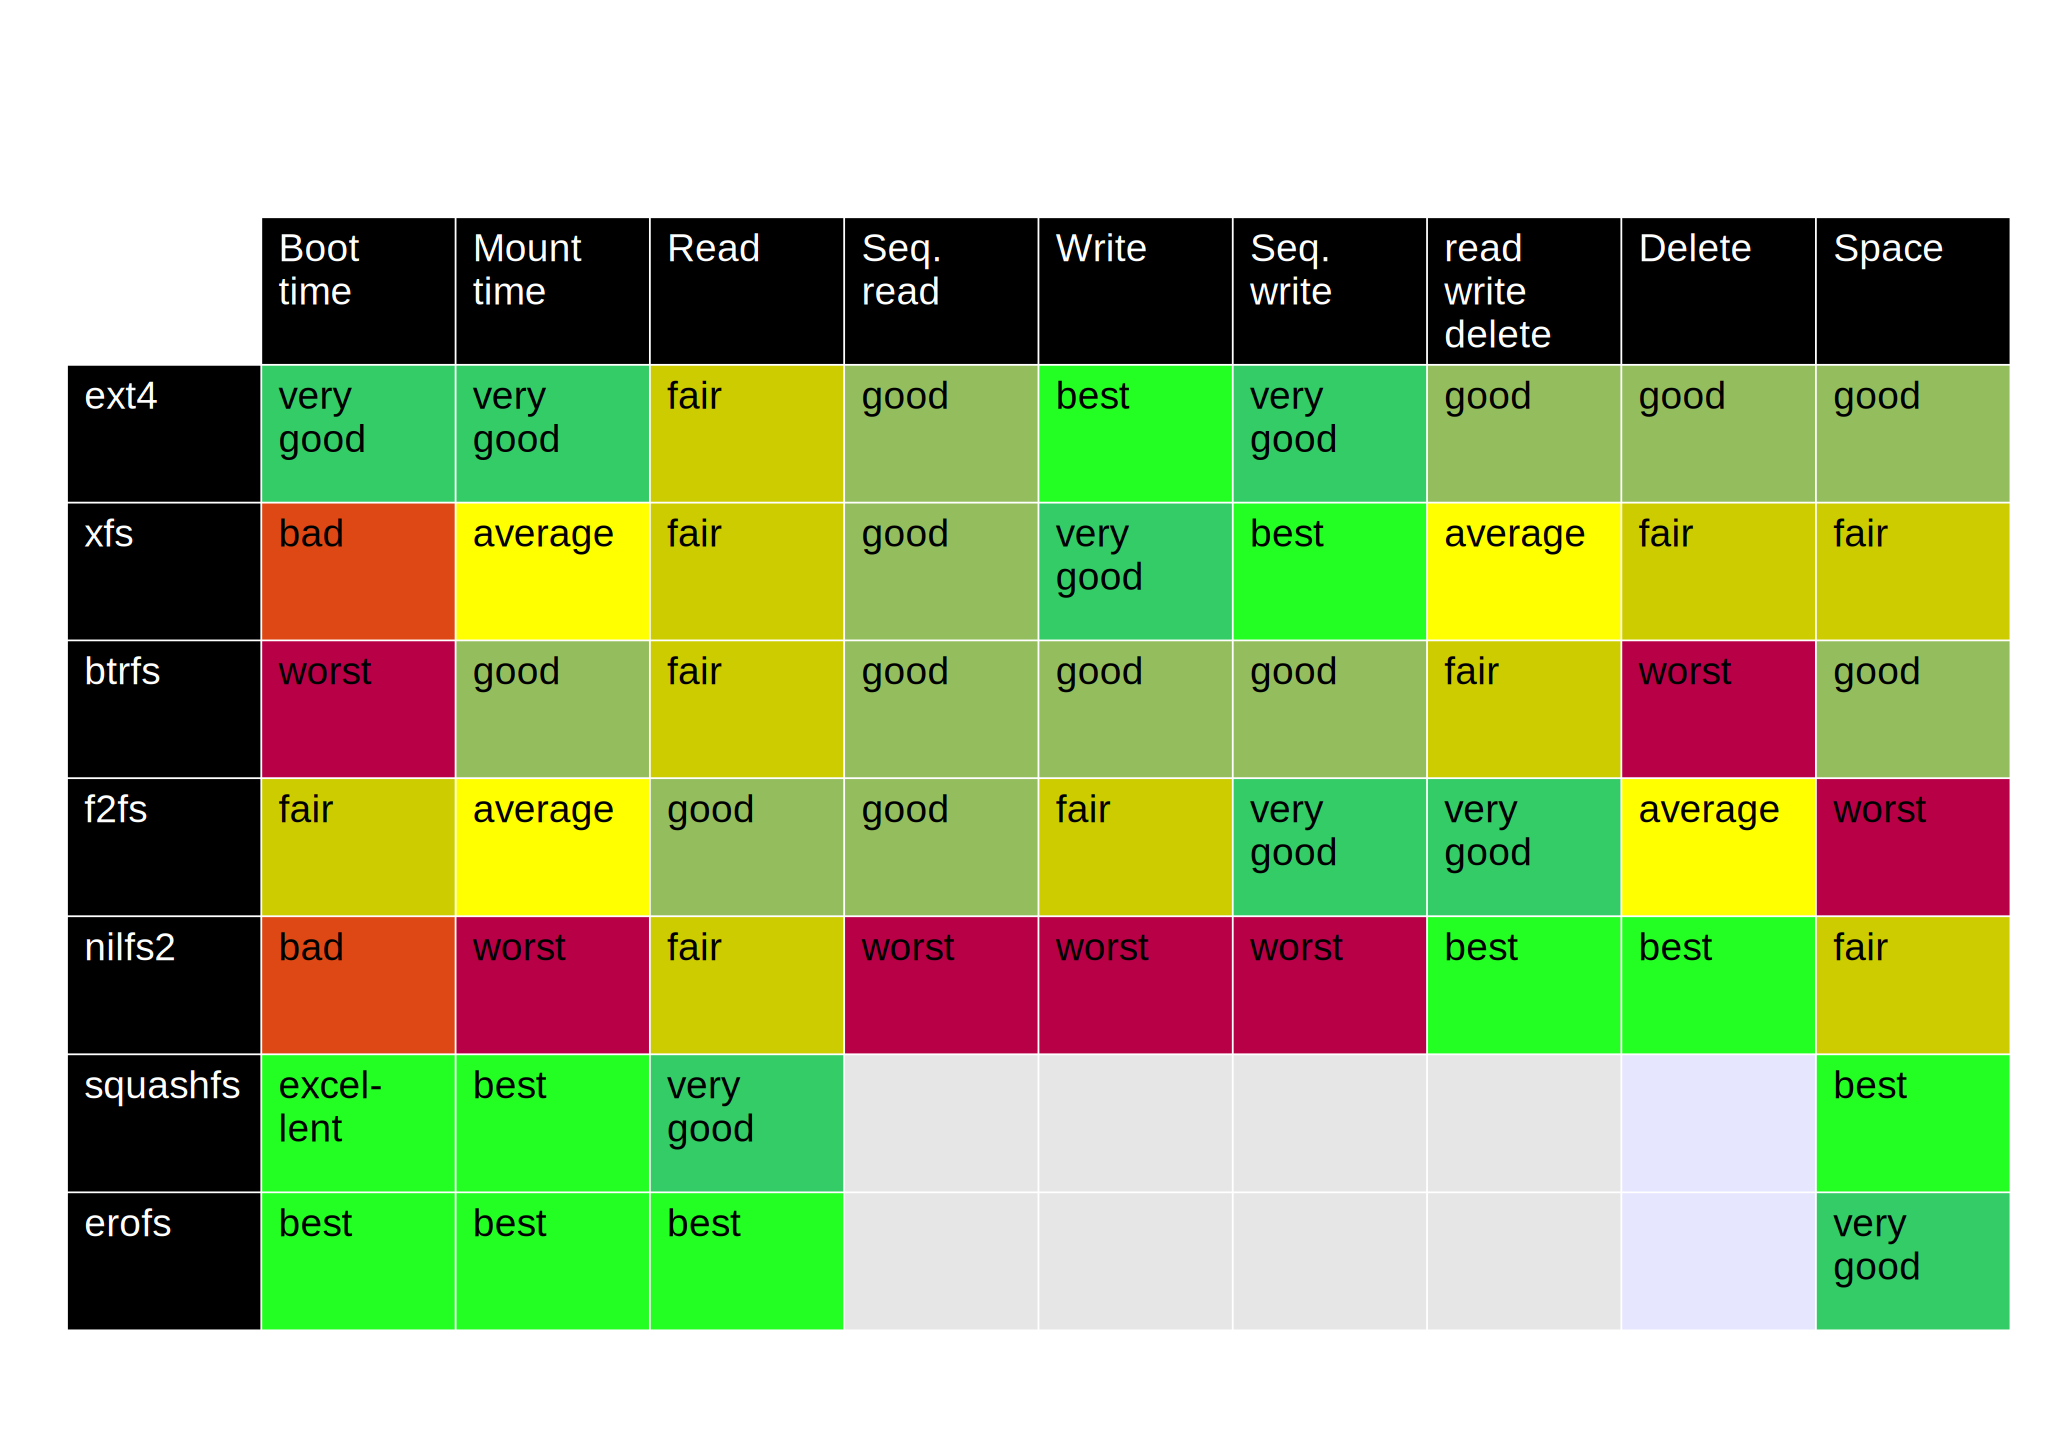
\includegraphics[height=0.7\textheight]{slides/sysdev-block-filesystems/rating.pdf}\\
  \small
  See our presentation for more details and benchmarks (Linux 6.3, ARM32 BeagleBone Black):
  \scriptsize
  \url{https://bootlin.com/pub/conferences/2023/eoss/opdenacker-finding-best-block-filesystem/}
\end{frame}

\begin{frame}
  \frametitle{Compatibility filesystems}
  Linux also supports several other filesystem formats, mainly to be
  interoperable with other operating systems:
  \begin{itemize}
  \item \code{vfat} (\kconfig{CONFIG_VFAT_FS}) for compatibility with the FAT filesystem used in
    the Windows world and on numerous removable devices
    \begin{itemize}
    \item Also convenient to store bootloader binaries (FAT easy
      to understand for ROM code)
    \item This filesystem does {\em not} support features like
      permissions, ownership, symbolic links, etc. Cannot be used for
      a Linux root filesystem.
    \item Linux now supports the exFAT filesystem too (\kconfig{CONFIG_EXFAT_FS}).
    \end{itemize}
  \item \code{ntfs} (\kconfig{CONFIG_NTFS_FS}) for compatibility with
      Windows NTFS filesystem.
  \item \code{hfs} (\kconfig{CONFIG_HFS_FS}) for compatibility with the
      MacOS HFS filesystem.
  \end{itemize}
\end{frame}

\begin{frame}
  \frametitle{tmpfs: filesystem in RAM}
  \kconfig{CONFIG_TMPFS}
  \begin{itemize}
  \item Not a block filesystem of course!
  \item Perfect to store temporary data in RAM: system log files,
    connection data, temporary files...
  \item More space-efficient than ramdisks: files are directly in the
    file cache, grows and shrinks to accommodate stored files
  \item How to use: choose a name to distinguish the various tmpfs
    instances you have (unlike in most other filesystems, each
    tmpfs instance is different). Examples:\\
    \code{mount -t tmpfs run /run}\\
    \code{mount -t tmpfs shm /dev/shm}
  \item See \kdochtml{filesystems/tmpfs} in kernel documentation.
  \end{itemize}
\end{frame}

\subsection{Using block filesystems}

\begin{frame}
  \frametitle{Creating filesystems}
  \begin{itemize}
  \item To create an empty ext4 filesystem on a block device or
    inside an already-existing image file
    \begin{itemize}
    \item \code{mkfs.ext4 /dev/sda3}
    \item \code{mkfs.ext4 disk.img}
    \end{itemize}
  \item To create a filesystem image from a directory containing all
    your files and directories
    \begin{itemize}
    \item For some filesystems, there are utilities to create a
          filesystem image from an existing directory:
          \begin{itemize}
          \item {\em ext2}: \code{genext2fs -d rootfs/ rootfs.img}
	      \item {\em squashfs}: \code{mksquashfs rootfs/ rootfs.sqfs} (details later)
          \item {\em erofs}: \code{mkfs.erofs rootfs.erofs rootfs/}
          \end{itemize}
    \item For other (read-write) filesystems: create a disk image,
          format it, mount it (see next slides), copy contents and umount.
    \item Your image is then ready to be transferred to your block device
    \end{itemize}
  \end{itemize}
\end{frame}

\begin{frame}
  \frametitle{Mounting filesystem images}
  \begin{itemize}
  \item Once a filesystem image has been created, one can access and
    modify its contents from the development workstation, using the
    {\bf loop} mechanism:
  \item Example:\\
    \code{mkdir /mnt/test}\\
    \code{mount -t ext4 -o loop rootfs.img /mnt/test}
  \item In the \code{/mnt/test} directory, one can access and modify
    the contents of the \code{rootfs.img} file.
  \item This is possible thanks to \code{loop}, which is a kernel
    driver that emulates a block device with the contents of a file.
  \item Note: \code{-o loop} no longer necessary with recent versions
        of \code{mount} from {\em GNU Coreutils}. Not true with BusyBox
       \code{mount}.
  \item Do not forget to run \code{umount} before using the filesystem
    image!
  \end{itemize}
\end{frame}

\begin{frame}[fragile]
  \frametitle{How to access partitions in a disk image}
  \begin{itemize}
  \item You may have dumped a complete block device (with partitions) into a disk image.
  \item The \code{losetup} command allows to manually associate
    a loop device to a file, and offers a \code{--partscan} option
    allowing to also create extra block device files for the partitions
    inside the image:
    \begin{block}{}
    \begin{verbatim}
$ sudo losetup -f --show --partscan disk.img
/dev/loop2

$ ls -la /dev/loop2*
brw-rw---- 1 root disk   7,  2 Jan 14 10:50 /dev/loop2
brw-rw---- 1 root disk 259, 11 Jan 14 10:50 /dev/loop2p1
brw-rw---- 1 root disk 259, 12 Jan 14 10:50 /dev/loop2p2
\end{verbatim}
    \end{block}{}
  \item Each partition can then be accessed individually, for example:
    \begin{block}{}
    \begin{verbatim}
$ mount /dev/loop2p2 /mnt/rootfs
\end{verbatim}
    \end{block}{}
  \end{itemize}
\end{frame}

\begin{frame}
  \frametitle{Creating squashfs filesystems}
  \begin{itemize}
  \item Need to install the \code{squashfs-tools} package
  \item Can only create an image: creating an empty {\em squashfs}
    filesystem would be useless, since it's read-only.
  \item To create a {\em squashfs} image:
    \begin{itemize}
    \item \code{mksquashfs data/ data.sqfs -noappend}
    \item \code{-noappend}: re-create the image from scratch rather
      than appending to it
    \end{itemize}
  \item Examples mounting a squashfs filesystem:
    \begin{itemize}
    \item Same way as for other block filesystems
    \item \code{mount -o loop data.sqfs /mnt} (filesystem image on the host)
    \item \code{mount /dev/<device> /mnt} (on the target)
    \end{itemize}
  \end{itemize}
\end{frame}

\begin{frame}
  \frametitle{Mixing read-only and read-write filesystems}
  \begin{columns}
    \column{0.8\textwidth}
    Good idea to split your block storage into:
    \begin{itemize}
    \item A compressed read-only partition (\code{SquashFS})\\
      Typically used for the root filesystem (binaries, kernel...).\\
      Compression saves space. Read-only access protects your system
      from mistakes and data corruption.
    \item A read-write partition with a journaled filesystem (like \code{ext4})\\
      Used to store user or configuration data.\\
      Journaling guarantees filesystem integrity after power off or crashes.
    \item Ram storage for temporary files (\code{tmpfs})
    \end{itemize}
    \column{0.2\textwidth}
    \includegraphics[height=0.8\textheight]{slides/sysdev-block-filesystems/mixing-filesystems.pdf}
  \end{columns}
\end{frame}

\begin{frame}
  \frametitle{Issues with flash-based block storage}
  \begin{itemize}
  \item Flash storage made available only through a block interface.
  \item Hence, no way to access a low level flash interface
    and use the Linux filesystems doing wear leveling.
  \item No details about the layer (Flash Translation Layer) they
    use. Details are kept as trade secrets, and may hide poor
    implementations.
  \item Not knowing about the wear leveling algorithm, it is highly
    recommended to limit the number of writes to these devices.
  \item Using industrial grade storage devices (MMC/SD, USB) is
    also recommended.
  \end{itemize}
  See the \href{https://lwn.net/Articles/428584/}{\em Optimizing Linux with
  cheap flash drives} article from Arnd Bergmann and try his {\em
  flashbench} tool (\url{http://git.linaro.org/people/arnd/flashbench.git/about/})
  for finding out the erase block and page size for your storage, and
  optimizing your partitions and filesystems for best performance.
  Note that some SD cards report their erase block size, available in
  \code{/sys/bus/mmc/devices/<dev>/preferred_erase_size}.
\end{frame}

\setuplabframe
{Block filesystems}
{
  \begin{itemize}
  \item Creating further partitions on your SD card
  \item Booting a system with a mix of filesystems: {\em SquashFS} for
    the root filesystem, {\em ext4} for data, and {\em
    tmpfs} for temporary system files.
  \item Loading everything from the SD card, including
    the kernel and device tree.
  \end{itemize}
}
